\documentclass[
  bibliography=totoc,     % Literatur im Inhaltsverzeichnis
  captions=tableheading,  % Tabellenüberschriften
  titlepage=firstiscover, % Titelseite ist Deckblatt
]{scrartcl}

% Paket float verbessern
\usepackage{scrhack}

% Warnung, falls nochmal kompiliert werden muss
\usepackage[aux]{rerunfilecheck}

% unverzichtbare Mathe-Befehle
\usepackage{amsmath}
% viele Mathe-Symbole
\usepackage{amssymb}
% Erweiterungen für amsmath
\usepackage{mathtools}

% Fonteinstellungen
\usepackage{fontspec}
% Latin Modern Fonts werden automatisch geladen
% Alternativ:
%\setromanfont{Libertinus Serif}
%\setsansfont{Libertinus Sans}
%\setmonofont{Libertinus Mono}
\recalctypearea % Wenn man andere Schriftarten gesetzt hat,
% sollte man das Seiten-Layout neu berechnen lassen

% deutsche Spracheinstellungen
\usepackage{polyglossia}
\setmainlanguage{german}


\usepackage[
  math-style=ISO,    % ┐
  bold-style=ISO,    % │
  sans-style=italic, % │ ISO-Standard folgen
  nabla=upright,     % │
  partial=upright,   % ┘
  warnings-off={           % ┐
    mathtools-colon,       % │ unnötige Warnungen ausschalten
    mathtools-overbracket, % │
},                       % ┘
]{unicode-math}

% traditionelle Fonts für Mathematik
\setmathfont{Latin Modern Math}
% Alternativ:
%\setmathfont{Libertinus Math}

\setmathfont{XITS Math}[range={scr, bfscr}]
\setmathfont{XITS Math}[range={cal, bfcal}, StylisticSet=1]

% Zahlen und Einheiten
\usepackage[
locale=DE,                   % deutsche Einstellungen
separate-uncertainty=true,   % immer Fehler mit \pm
per-mode=symbol-or-fraction, % / in inline math, fraction in display math
alsoload=<torr>
]{siunitx}

% chemische Formeln
\usepackage[
version=4,
math-greek=default, % ┐ mit unicode-math zusammenarbeiten
text-greek=default, % ┘
]{mhchem}

% richtige Anführungszeichen
\usepackage[autostyle]{csquotes}

% schöne Brüche im Text
\usepackage{xfrac}
\usepackage{tabularx}
% Standardplatzierung für Floats einstellen
\usepackage{float}
\floatplacement{figure}{htbp}
\floatplacement{table}{htbp}

% Floats innerhalb einer Section halten
\usepackage[
section, % Floats innerhalb der Section halten
below,   % unterhalb der Section aber auf der selben Seite ist ok
]{placeins}

% Seite drehen für breite Tabellen: landscape Umgebung
\usepackage{pdflscape}

% Captions schöner machen.
\usepackage[
  labelfont=bf,        % Tabelle x: Abbildung y: ist jetzt fett
  font=small,          % Schrift etwas kleiner als Dokument
  width=0.9\textwidth, % maximale Breite einer Caption schmaler
]{caption}
% subfigure, subtable, subref
\usepackage{subcaption}

% Grafiken können eingebunden werden
\usepackage{graphicx}
% größere Variation von Dateinamen möglich
\usepackage{grffile}

% schöne Tabellen
\usepackage{booktabs}

% Verbesserungen am Schriftbild
\usepackage{microtype}

% Literaturverzeichnis
\usepackage[style=alphabetic,]{biblatex}
% Quellendatenbank
\addbibresource{lit.bib}

% Hyperlinks im Dokument
\usepackage[
  unicode,        % Unicode in PDF-Attributen erlauben
  pdfusetitle,    % Titel, Autoren und Datum als PDF-Attribute
  pdfcreator={},  % ┐ PDF-Attribute säubern
  pdfproducer={}, % ┘
]{hyperref}
% erweiterte Bookmarks im PDF
\usepackage{bookmark}

% Trennung von Wörtern mit Strichen
\usepackage[shortcuts]{extdash}

\title{V503: Der Millikan-Öltröpfchenversuch}
\author{
  Simon Schulte
  \texorpdfstring{
    \\
    \href{mailto:simon.schulte@udo.edu}{simon.schulte@udo.edu}
  }{}
  \texorpdfstring{\and}{, }
  Tim Sedlaczek
  \texorpdfstring{
    \\
    \href{mailto:tim.sedlaczek@udo.edu}{tim.sedlaczek@udo.edu}
  }{}
}
\publishers{TU Dortmund – Fakultät Physik}

\date{Durchführung: 16.05.2017\\
      Abgabe: 23.05.2017}


\begin{document}

\maketitle
\thispagestyle{empty}
\tableofcontents
\newpage
\setcounter{page}{1}
\section{Zielsetzung}
\label{sec:zielsetzung}
Bei dem Millikan-Öltröpfchenversuch wir anhand der Bewegungen
eines geladenen Öltröpfchens im Feld eines Plattenkondensators.
Die Elementarladung bestimmt.

\noindent
Bei dem regulären Verfahren wird dazu die Geschwindigkeit des Tröpfchens,
für einen abgeschalteten Kondensator und für die zwei verschiedenen
Möglichkeiten der Polarisierung des Kondensators, bei bekannten Spannungen
gemessen.
Hier wird jedoch ein leicht verändertes Verfahren verwendet.
\section{Theorie}
\label{sec:theorie}
Beim einsprühen des Öls in die Apparatur werden die Öltröpfchen
durch Reibung geladen. Zwischen den Kondensatorplatten
erfahren sie dann mehrere Kräfte:

\noindent
Die Gewichtskraft
\begin{equation}
  \vec{F}_ \mathup{g} = m \cdot \vec{g},
\end{equation}
die Stokesche Reibung
\begin{equation}
  \vec{F}_\mathup{R} = - 6 \pi r \eta_\mathup{L} \vec{v}
\end{equation}
und, bei eingeschaltetem Kondensator, die elektrische Kraft
\begin{equation}
  \vec{F}_\mathup{el} = q \cdot \vec{E}.
\end{equation}
$g$ ist dabei die Schwerebeschleunigung, $r$ der Radius des Tröpfchens, $\eta_\mathup{L}$
die Viskosität der Luft und $E$ die elektrische Feldstärke im Kondensator.

\noindent
Bei einem Kräftegleichgewicht bewegen sich die Tröpfchen mit konstanter
Geschwindigkeit $v$.
Zunächst wird das Gleichgewicht bei abgeschaltetem Kondensator betrachtet.
Dabei sind die Gewichtskraft und die Stokesche Reibung betragsweise gleich
groß. Durch umschreiben der Masse $m$ in ein Produkt aus Dichte $\rho$ und
Volumen $\frac{4 \pi}{3}r^3$ folgt:
\begin{equation}
  \frac{4 \pi}{3}r^3 \rho g = 6 \pi \eta_\mathup{L} r v_0.
  \label{eqn:kräftegleichgew}
\end{equation}
Daraus folgt der Tröpfchenradius
\begin{equation}
  r = \sqrt{\frac{9 \eta_\mathup{L} v_0}{2 g \rho}}.
  \label{eqn:tröpfchenradius}
\end{equation}
Zur Bestimmung der Ladung wird der Kondensator eingeschaltet und eine ausreichend
große Spannung angelegt, sodass das Tröpfchen in der Luft schwebt. In diesem Fall
sind die elektrische Kraft und die Gewichtskraft im Gleichgewicht:
\begin{equation}
  \frac{4 \pi}{3}r^3 \rho g = q \cdot E = q \cdot \frac{U}{d}
  \label{eqn:gleichgewicht}
\end{equation}
Daraus folgt die Ladung des Tröpfchens
\begin{equation}
  q = \frac{4 \pi}{3}r^3 \rho g \frac{d}{U}
  \label{eqn:ladung}
\end{equation}

\noindent
Da die Stokesche Reibung so wie sie bisher verwendet wurde nur für Tröpfchen gilt,
die größer sind als die mittlere freie Weglänge in Luft, muss die Viskosität
der Luft korrigiert werden:
\begin{equation}
  \eta_{eff} = \eta_\mathup{L} \Biggl( \frac{1}{1+\frac{B}{pr}} \Biggr).
  \label{eqn:1}
\end{equation}
Hierbei ist $B = \SI{6.17e-3}{\torr\centi\meter}$ und $p$ der Luftdruck.
Daraus ergibt sich die korrigierte Ladung
\begin{equation}
  q_\mathup{Korr} = q_0 \biggl( 1 + \frac{B}{pr} \biggr)^{-\frac{3}{2}}.
  \label{eqn:2}
\end{equation}
\section{Durchführung}
\label{sec:durchführung}
\subsection{Versuchsaufbau}
\begin{figure}[htb]
  \centering
  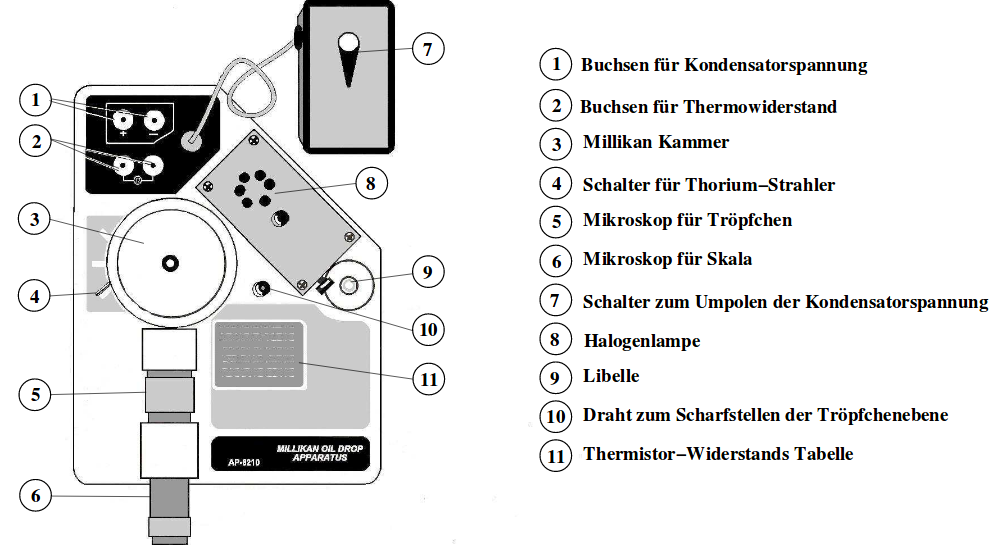
\includegraphics[width=0.9\textwidth]{5031.png}
  \caption{Der Versuchsaufbau. \cite{anleitung}}
  \label{fig:5031}
\end{figure}
In Abbildung \ref{fig:5031} ist der Aufbau der Apparatur für den Millikanversuch
dargestellt.

\noindent
An den Buchsen 1 und 2 kann die tatsächlich am Kondensator anliegende Spannung
und der thermische/elektrische Widerstand der Luft gemessen werden.
Über den Widerstand wird dann während des Versuchs die Temperatur im Innern des
Kondensators bestimmt. Für den Fall, dass die Öltröpfchen nicht hinreichend geladen sein sollten,
ist ein Alphastrahler in die Apparatur integriert. Dieser ist von der Kammer abgeschirmt.
Um dir Abschirmung kurzzeitig zu entfernen kann der Hebel 4 in die "On" Stellung
gelegt werden. Mit dem Mikroskop wird das Innere der Kammer aufgenommen und auf
einem Bildschirm angezeigt. Das Bild kann an dem Mikroskop auf die Tröpfchenebene
und auf die Skala fokussiert werden. Damit die Tröpfchen nicht seitlich abdriften
muss die Apparatur möglichst gerade ausgerichtet sein. Die Libelle 9 zeigt dabei
die Neigung an.
\subsection{Versuchsablauf}
Zu Beginn der Messung wird an der Oberseite, der Millikan Kammer, Öl zerstäubt.
An dem Bildschirm können dann die Tröpfchen beobachtet werden.

\noindent
Führ die Messung wird ein relativ langsames Tröpfchen gewählt.
Durch einschalten des Kondensators wird geprüft ob das Tröpfchen
geladen ist. Wenn sich ein Tröpfchen entsprechend für die Messung
eignet wird die Zeit gestoppt, die es bei abgeschaltetem Kondensator
benötigt, um $\SI{0.5}{\milli\meter}$ zurückzulegen. Anschließend wird
mit dem Generator eine Spannung eingestellt, die so groß ist, dass das
Tröpfchen in der Luft ruht. Die eingestellte Spannung wird dann zusammen
mit der aktuellen Temperatur in der Kammer notiert.

\noindent
Wenn keine passenden Tröpfchen auf dem Bild zu sehen sind kann durch
Pusten dafür gesorgt werden, dass neue Öltröpfchen vor das Mikroskop
gelangen. Sollte dies nicht weiter helfen wird neues Öl in der Kammer
zerstäubt. Die Messung der Fallzeit, der Spannung und der Temperatur
wird für $25$ Tröpfchen durchgeführt.
\clearpage

\section{Auswertung}
\label{sec:auswertung}
Die in der Auswertung verwendeten Mittelwerte mehrfach gemessener Größen sind gemäß der
Gleichung
%
\begin{equation}
    \bar{x}=\frac{1}{n}\sum_{i=1}^n x_i
    \label{eq:mittelwert}
\end{equation}

bestimmt. Die Standardabweichung des Mittelwertes ergibt sich dabei zu

\begin{equation}
    \mathup{\Delta}\bar{x}=\sqrt{\frac{1}{n(n-1)}\sum_{i=1}^n\left(x_i-\bar{x}\right)^2}.
    \label{eq:standardabweichung}
\end{equation}

Resultiert eine Größe über eine Gleichung aus zwei oder mehr anderen fehlerbehafteten Größen, so
berechnet sich der Gesamtfehler nach der Gaußschen Fehlerfortpflanzung zu

\begin{equation}
    \mathup{\Delta}f(x_1,x_2,...,x_n)=\sqrt{\left(\frac{\partial f}{\partial x_1}\mathup{\Delta}x_1\right)^2+\left(\frac{\partial f}{\partial x_2}\mathup{\Delta}x_2\right)^2+ \dotsb +\left(\frac{\partial f}{\partial x_n}\mathup{\Delta}x_n\right)^2}.
    \label{eq:fehlerfortpflanzung}
\end{equation}

Alle in der Auswertung angegebenen Größen sind stets auf die erste signifikante Stelle des
Fehlers gerundet. Setzt sich eine Größe über mehrere Schritte aus anderen Größen zusammen,
so wird erst am Ende gerundet, um Fehler zu vermeiden. Zur Auswertung wird das Programm Python verwendet.
\subsection{Bestimmung der Tröpfchenladung \texorpdfstring{$q$}{q}}

Zur Bestimmung der Elementarladung $\epsilon_0$ werden insgesamt 25 Tröpfchen beobachtet. Die Tabelle~\ref{tab:messwerte1} zeigt die aufgenommenen Messwerte. Die in den jeweiligen Zeiten zurückgelegte Strecke beträgt jeweils $\SI{0.5}{\milli\metre}$. Es wird die Zeit $t_0$, aus der sich die Geschwindigkeit $v_0$ ergibt, die Temperatur $T$, die sich aus dem Thermowiderstand ergibt und die Spannung, bei der sich das jeweilige Tröpfchen nicht mehr bewegt hat, angegeben.

\begin{table}[H]
	\begin{center}
	\caption{Die Messwerte der 25 Tröpfchen.}
	\label{tab:messwerte1}
		\begin{tabular}{cccc}
			\toprule
			{Nr.} & {$t_0$} {[$\si{\second}$]} & {$U$ [$\si{\volt}$]}
      & {$T$ [$\si{\celsius}$]}\\
			\midrule
			1  & $37.724$ & $17.6$ & $26$ \\
			2  & $14.577$ & $55.5$ & $26$ \\
			3  & $16.949$ & $26.3$ & $27$ \\
			4  & $18.593$ & $27.2$ & $27$ \\
			5  & $26.293$ & $157.6$ & $28$ \\
			6  & $11.280$ & $225.0$ & $29$ \\
			7  & $27.460$ & $127.0$ & $29$ \\
			8  & $17.560$ & $180.0$ & $29.5$ \\
			9  & $48.204$ & $16.0$ & $30$ \\
			10 & $11.264$ & $50.0$ & $30$ \\
			11 & $16.524$ & $81.0$ & $30$ \\
			12 & $22.679$ & $72.0$ & $30.5$ \\
			13 & $24.099$ & $69.0$ & $31$ \\
			14 & $30.833$ & $92.0$ & $31$ \\
			15 & $14.606$ & $102.0$ & $31$ \\
			16 & $40.480$ & $57.0$ & $31.5$ \\
			17 & $33.192$ & $49.0$ & $31.5$ \\
			18 & $21.125$ & $84.0$ & $32$ \\
			19 & $13.440$ & $179.0$ & $32$ \\
			20 & $12.866$ & $144.0$ & $32$ \\
			21 & $12.301$ & $121.0$ & $32$ \\
			22 & $12.633$ & $153.0$ & $32$ \\
			23 & $16.055$ & $77.0$ & $32$ \\
			24 & $13.559$ & $88.0$ & $32$ \\
			25 & $15.533$ & $183.0$ & $32$ \\
			\bottomrule
		\end{tabular}
	\end{center}
\end{table}

Nun werdem mit Hilfe der Gleichungen~\eqref{eqn:ladung} und~\eqref{eqn:tröpfchenradius}, Radius und Ladung der Tröpfchen ermittelt. Zur Bestimmung der temperaturabhängigen Viskosität $\eta_{\mathup{L}}$ von Luft, die im relevanten Temperaturbereich zwischen $\SI{26}{\celsius}$ und $\SI{32}{\celsius}$ annähernd linear verläuft, werden die Werte aus dem in \cite{anleitung} gegebenen Graphen abgelesen.
 Die Bestimmung der Temperatur aus dem gemessenen Thermistorwiderstand der Apparatur erfolgt mit Hilfe einer Widerstandstabelle, die sich auf einem der Versuchsgeräte befand. Tabelle~\ref{tab:ergebnisse} listet die Radien und Ladungen der Tröpfchen auf. Bei der angegebenen Ladung $q_{\mathup{k}}$ handelt es sich um die nach Cunnigham korrigierte Ladung. Der Zusammenhang zwischen korrigierter Ladung $q_{\mathup{k}}$ erfolgt aus den Gleichungen~\eqref{eqn:1} und~\eqref{eqn:2}.
\begin{table}[H]
        \begin{center}
        \captionsetup{width=\linewidth}
        \captionof{table}{Ergebnisse der Berechnung zur Bestimmung der Ladung eines Öltröpfchens.}
        \label{tab:ergebnisse}
            \begin{tabular}{
                    S[table-format =  2.0]
                    S[table-format =  1.3]
                    S[table-format =  1.2]
                    S[table-format =  2.2]
                    S[table-format =  2.2]
                    S[table-format =  2.2]
                    S[table-format =  2.2]
                    S[table-format =  2.0]
                    S[table-format =  2.0]
                    }
                \toprule
                {Nr.} &
                {$\eta_{\mathup{L}}$} &
                {$r$} &
                {$q$} &
                {$\mathup{\Delta}q$} &
                {$q_{k}$} &
                {$\mathup{\Delta}q_{k}$} \\
                \midrule
                {} &
                {[$\SI{e-5}{\newton\second\per\metre\squared}$]} &
                {[$\SI{e-7}{\metre}$]} &
                {[$\SI{e-19}{\coulomb}$]} &
                {[$\SI{e-22}{\coulomb}$]} &
                {[$\SI{e-19}{\coulomb}$]} &
                {[$\SI{e-22}{\coulomb}$]} \\
                \midrule
                 1 & 1.853 & 3.56 & 7.15 & 4.78 & 5.26 & 3.52 \\
                 2 & 1.853 & 5.73 & 9.44 & 6.32 & 7.74 & 5.18 \\
                 3 & 1.858 & 5.32 & 15.9 & 10.7 & 12.9 & 8.63 \\
                 4 & 1.858 & 5.08 & 13.4 & 8.98 & 10.8 & 7.20 \\
                 5 & 1.862 & 4.28 & 1.38 & 0.92 & 1.07 & 0.71 \\
                 6 & 1.867 & 6.54 & 3.46 & 2.31 & 2.90 & 1.94 \\
                 7 & 1.867 & 4.19 & 1.61 & 1.08 & 1.24 & 0.83 \\
                 8 & 1.869 & 5.24 & 2.23 & 1.49 & 1.80 & 1.20 \\
                 9 & 1.872 & 3.17 & 5.53 & 3.70 & 3.93 & 2.63 \\
                10 & 1.872 & 6.56 & 15.6 & 10.5 & 13.2 & 8.80 \\
                11 & 1.872 & 5.41 & 5.44 & 3.64 & 4.42 & 2.95 \\
                12 & 1.874 & 4.62 & 3.81 & 2.55 & 2.99 & 2.00 \\
                13 & 1.876 & 4.48 & 3.64 & 2.43 & 2.84 & 1.90 \\
                14 & 1.876 & 3.96 & 1.88 & 1.26 & 1.43 & 0.95 \\
                15 & 1.876 & 5.76 & 5.21 & 3.49 & 4.28 & 2.87 \\
                16 & 1.878 & 3.46 & 2.02 & 1.36 & 1.48 & 1.00 \\
                17 & 1.878 & 3.82 & 3.17 & 2.12 & 2.38 & 1.59 \\
                18 & 1.881 & 4.80 & 3.65 & 2.45 & 2.89 & 1.94 \\
                19 & 1.881 & 6.02 & 3.38 & 2.26 & 2.80 & 1.87 \\
                20 & 1.881 & 6.15 & 4.48 & 3.00 & 3.73 & 2.49 \\
                21 & 1.881 & 6.29 & 5.71 & 3.82 & 4.76 & 3.19 \\
                22 & 1.881 & 6.20 & 4.34 & 2.90 & 3.61 & 2.42 \\
                23 & 1.881 & 5.50 & 6.02 & 4.03 & 4.90 & 3.28 \\
                24 & 1.881 & 5.99 & 6.79 & 4.54 & 5.61 & 3.75 \\
                25 & 1.881 & 6.00 & 2.66 & 1.78 & 2.17 & 1.45 \\
                \bottomrule
            \end{tabular}
        \end{center}
    \end{table}
\newpage
Ein Blick auf die errechneten Werte für
$q_{\mathup{k}}$ und $q$ zeigt, dass diese zum größten Teil von einer ganzen Zahl abweichen.
Da solche Werte für die weitere Auswertung nicht zu gebrauchen sind, werden im Folgenden nur die Werte verwendet, die einen relativen Fehler $\leq\SI{20}{\percent}$ haben. Damit scheiden alle Tröpfchen außer 2, 3, 5, 6, 7, 14, 17, 19, und 20 aus. \ref{tab:elementarladungen} zeigt die einzelnen Elementarladungen dieser Tröpfchen und die Faktoren, durch die jeweils geteilt werden musste.
\begin{table}[H]
        \begin{center}
        \captionsetup{width=\linewidth}
        \captionof{table}{Faktoren und daraus resultierende Elementarladungen.}
        \label{tab:elementarladungen}
            \begin{tabular}{
                    S[table-format =  2.0]
                    S[table-format =  2.0]
                    S[table-format =  1.2]
                    S[table-format =  2.0]
                    S[table-format =  1.2]
                    }
                \toprule
                {Nr.} &
                {Faktor für $q$} &
                {$e$} &
                {Faktor für $q_k$} &
                {$e_k$} \\
                \midrule
                {} &
                {} &
                {[$\SI{e-19}{\coulomb}$]} &
                {} &
                {[$\SI{e-19}{\coulomb}$]} \\
                \midrule
                 2 & 6 & 1.57 & 5 & 1.55\\
                 3 & 10 & 1.60 & 8 & 1.61\\
                 5 & 1 & 1.38 & 1 & 1.07\\
                 6 & 2 & 1.73 & 2 & 1.45\\
                 7 & 1 & 1.61 & 1 & 1.24\\
                14 & 1 & 1.89 & 1 & 1.43\\
                17 & 2 & 1.60 & 1 & 2.38\\
                19 & 2 & 1.69 & 2 & 1.40\\
                20 & 3 & 1.50 & 2 & 1.86\\
                \bottomrule
            \end{tabular}
        \end{center}
    \end{table}
Jetzt geht es nun darum, aus den übrigen Ladungen per Mittelwert die Elementarladung $\epsilon_0$ zu bestimmen.

Der Theorie nach sollten sich die Messpunkte in diskreten, horizontal gelegenen Abschnitten ("Balken") aufhalten, da es nur möglich ist die Elementarladung oder ganzzahlige Vielfache dieser zu messen. Eine kontinuierliche Verteilung der Messwerte widerspräche der Theorie. Daher werden in Abbildung~\ref{fig:messwerte} die gültigen Messpunkte des durchgeführten Versuchs aufgetragen. Das Problem ist nur, dass keine "Balken" zu erkennen sind.

\begin{figure}[h]
    \centering
    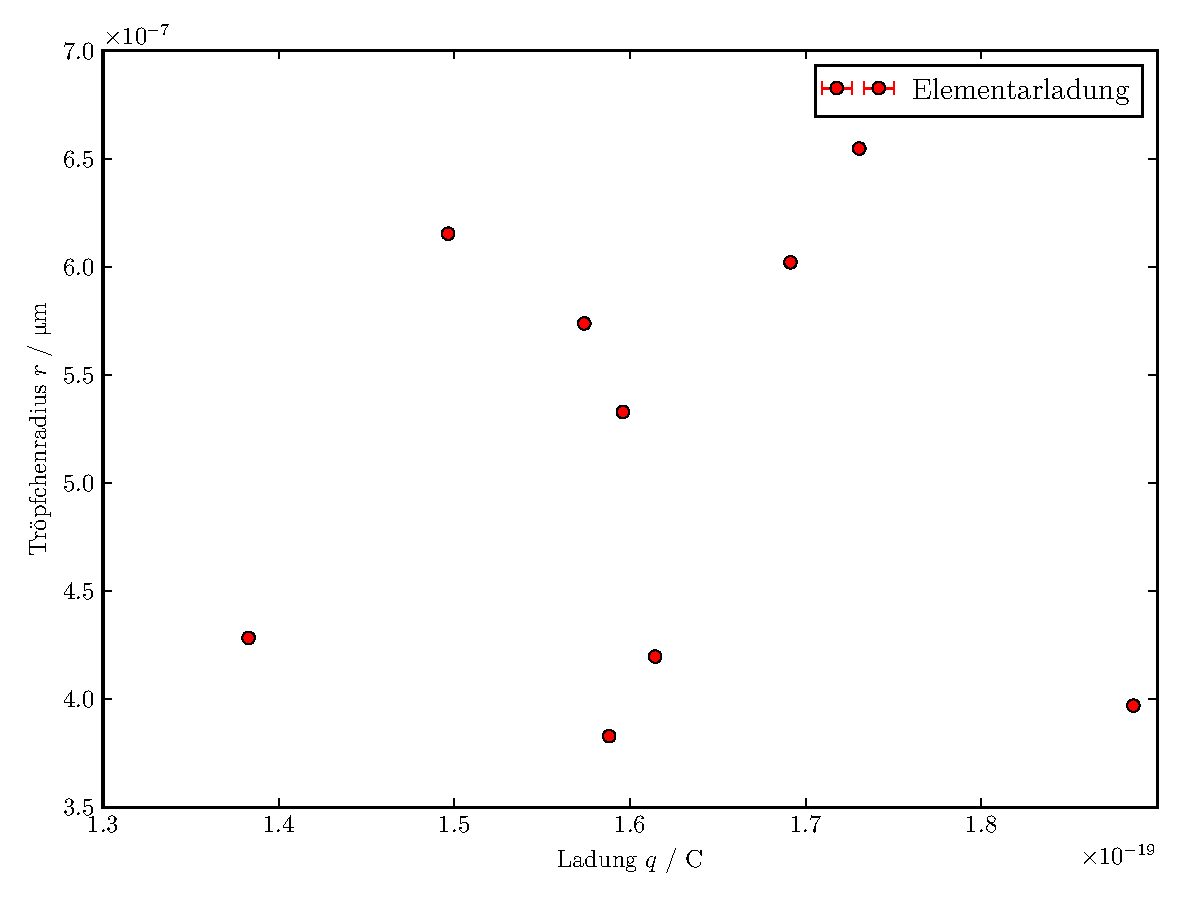
\includegraphics[width=0.9\textwidth]{plot_messwerte.pdf}
    \caption{Darstellung der unkorrigierten Ladungen der untersuchten Tröpfchen in Abhängigkeit des Tröpfchenradius.}
    \label{fig:messwerte}
\end{figure}

Aufgrund der Tatsache, dass die Ladung quantisiert ist und nur als Vielfache der Elementarladung $\epsilon_0$ auftreten kann, werden nun die in ~\ref{tab:ergebnisse} stehenden Ladungen durch die Elementarladung geteilt. Hierzu wird die in SciPy enthaltene Elementarladung verwendet. Als Mittel der betrachteten Tröpfchen ergibt sich dann für die nicht korrigierten Ladungen ein Wert von

\begin{equation}
    \epsilon_0 = \SI{1.62(5)e-19}{\coulomb}.
\end{equation}

Dieser Wert liegt sehr nah am Literaturwert $e = \SI{1.602e-19}{\coulomb}$ \cite{Elementarladung}. Abbildung~\ref{fig:messwerte+} zeigt nun die Punkte der korrigierten Ladung, die ebenso wie die errechneten nicht korrigierten Ladungen keine Balken darstellen. Für die Elementarladung der korrigierten Ladungen ergibt sich analog wie zuvor eine Elementarladung von

\begin{equation}
    \epsilon_0 = \SI{1.55(12)e-19}{\coulomb}.
\end{equation}
Auch dieser Wert liegt nah am Literaturwert.
\begin{figure}[h]
    \centering
    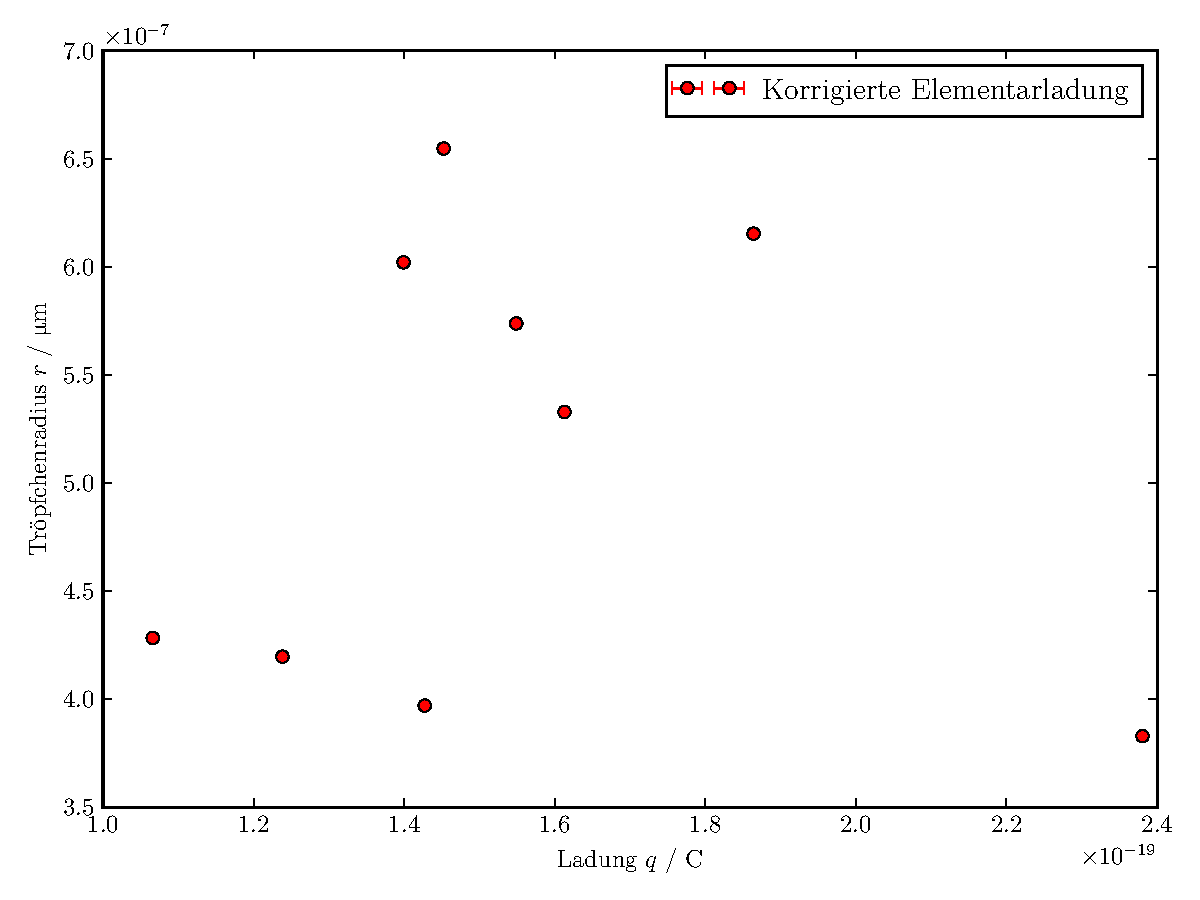
\includegraphics[width=0.9\textwidth]{plot_messwerte+.pdf}
    \caption{Darstellung der korrigierten Ladung der untersuchten Tröpfchen in Abhängigkeit des Tröpfchenradius mit eingezeichneten Vielfachen der errechneten Elementarladung.}
    \label{fig:messwerte+}
\end{figure}

\subsection{Bestimmung der Avogadro-Konstante}

In einem letzten Schritt soll noch von der errechneten Elementarladung mit Hilfe der Faraday-Konstante auf die Avogadro-Konstante geschlossen werden. Die benötigte Faraday-Konstante hat den Wert $F=\SI{96485.337}{\coulomb\per\mol}$~\cite{faraday} und ist die Ladung eines Mols einfach geladener Ionen. Dividiert durch die Elementarladung $\epsilon_0$ ergibt sich die Anzahl an Teilchen in einem Mol: die Avogadro-Konstante $N_{\mathup{A}}$. Es folgt für die nicht korrigierte Elementarladung

\begin{equation}
    N_{\mathup{A}}=\frac{F}{e}=\frac{\SI{96485.337}{\coulomb\per\mol}}{\SI{1.62e-19}{\coulomb}}=\SI{5.96e23}{\per\mol}.
\end{equation}

Damit liegt verständlicherweise auch dieser errechnete Wert nah am bekannten Literaturwert von $N_{\mathup{A}}=\SI{6.022e23}{\per\mol}$~\cite{avogadro}.

Für die korrigierte Elementarladung folgt
\begin{equation}
    N_{\mathup{A}}=\frac{F}{e}=\frac{\SI{96485.337}{\coulomb\per\mol}}{\SI{1.55e-19}{\coulomb}}=\SI{6.22e23}{\per\mol}.
\end{equation}
Auch dieser Wert für die Avogadro-Konstante liegt nahe am Literaturwert.
\section{Diskussion}
\label{sec:diskussion}

Der Versuch erweist sich in der Durchführung als schwierig. Messungen können häufig nicht zu Ende geführt werden oder müssen gar ganz verworfen werden. Der dadurch entstehende Mehraufwand an Zeit ist groß. Außerdem konnten lediglich 10 der 25 gemessenen Tröpfchen berücksichtigt werden, wenn man alle Tröpfchen mit einem relativen Fehler $\leq\SI{20}{\percent}$ betrachtet. Es ergibt sich damit ein Wert mit einer relativen Abweichung von ca. $\SI{1.2}{\percent}$, für die nicht korrigierte Ladung, und eine relative Abweichung von ca. $\SI{1}{\percent}$, für die korrigierte Ladung, vom Literaturwert. Die gut errechnete Elementarladung führt dann auch zu einer Avogadro-Konstante, die nahe am Literaturwert liegt. Insgesamt sind die Ergebnisse mit einer Abweichung von jeweils etwa $\SI{1}{\percent}$ vom jeweiligen Literaturwert sehr gut.

\nocite{*}
\printbibliography
\end{document}
